\documentclass[11pt]{article}

% =========================
% Packages
% =========================
\usepackage[margin=0.78in]{geometry}
\usepackage{amsmath,amssymb,amsfonts,mathtools}
\usepackage{booktabs,array,tabularx,longtable,multirow}
\usepackage{enumitem}
\usepackage[most]{tcolorbox}
\usepackage{xcolor}
\usepackage{fancyhdr}
\usepackage{titlesec}
\usepackage{hyperref}
\usepackage{lastpage}
\usepackage{setspace}
\usepackage{tikz}
\usepackage{pgfplots}
\usepackage{needspace}
\usepackage{caption}
\usepackage{multicol}
\usepackage{graphicx}
\usepackage{amsthm}
\usepackage{mathrsfs}
\usepackage{bm}
\usepackage{float}
\usetikzlibrary{calc,arrows.meta,positioning,decorations.pathreplacing,patterns}

\pgfplotsset{compat=1.18}
\setstretch{1.14}
\setlength{\parindent}{0pt}
\setlength{\parskip}{0.45em}
\setlist[itemize]{leftmargin=1.8em}
\setlist[enumerate]{leftmargin=2em}

% =========================
% Colors
% =========================
\definecolor{novelPurple}{RGB}{98,54,255}
\definecolor{novelPurpleDark}{RGB}{72,34,204}
\definecolor{novelPurpleLight}{RGB}{243,239,255}
\definecolor{novelPurpleLine}{RGB}{165,135,255}
\definecolor{npgray}{RGB}{78,78,78}
\definecolor{softgray}{RGB}{246,246,250}
\definecolor{softlav}{RGB}{249,247,255}
\definecolor{greencheck}{RGB}{24,128,88}
\definecolor{warmred}{RGB}{188,54,54}
\definecolor{nporange}{RGB}{223,121,36}
\definecolor{npgreen}{RGB}{67,142,103}
\definecolor{npred}{RGB}{180,54,54}

% =========================
% Hyperref
% =========================
\hypersetup{
    colorlinks=true,
    linkcolor=novelPurpleDark,
    urlcolor=novelPurpleDark,
    citecolor=novelPurpleDark
}

% =========================
% Header / Footer
% =========================
\pagestyle{fancy}
\fancyhf{}
\fancyhead[L]{\textbf{Novel Prep Learning Center}}
\fancyhead[R]{\textbf{AP Calculus AB/BC --- Unit 6}}
\fancyfoot[C]{\textcolor{novelPurpleDark}{\thepage\ /\ \pageref{LastPage}}}
\renewcommand{\headrulewidth}{0.4pt}
\renewcommand{\footrulewidth}{0pt}

% =========================
% Numbering / TOC
% =========================
\setcounter{secnumdepth}{3}
\setcounter{tocdepth}{3}

% =========================
% Section styles
% =========================
\titleformat{\section}
{\Large\bfseries\color{novelPurpleDark}}{\thesection.}{0.6em}{}

\titleformat{\subsection}
{\large\bfseries\color{novelPurple}}{\thesubsection.}{0.6em}{}

\titleformat{\subsubsection}
{\normalsize\bfseries\color{novelPurpleDark}}{\thesubsubsection.}{0.6em}{}

% =========================
% Boxes
% =========================
\tcbset{
  enhanced,
  sharp corners,
  boxrule=1pt
}

\newtcolorbox{theorybox}[1]{
  colback=white,
  colframe=novelPurple,
  colbacktitle=novelPurple,
  coltitle=white,
  title=\textbf{#1},
  fonttitle=\bfseries,
  sharp corners,
  breakable
}

\newtcolorbox{notebox}[1]{
  colback=novelPurpleLight,
  colframe=novelPurple,
  colbacktitle=novelPurple,
  coltitle=white,
  title=\textbf{#1},
  fonttitle=\bfseries,
  sharp corners,
  breakable
}

\newtcolorbox{skillbox}[1]{
  colback=softlav,
  colframe=novelPurpleDark,
  colbacktitle=novelPurpleDark,
  coltitle=white,
  title=\textbf{#1},
  fonttitle=\bfseries,
  sharp corners,
  breakable
}

\newtcolorbox{summarybox}[1]{
  colback=softgray,
  colframe=novelPurpleDark,
  colbacktitle=novelPurpleDark,
  coltitle=white,
  title=\textbf{#1},
  fonttitle=\bfseries,
  sharp corners,
  breakable
}

\newtcolorbox{practicebox}[1]{
  colback=white,
  colframe=novelPurpleLine,
  colbacktitle=novelPurpleLine,
  coltitle=black,
  title=\textbf{#1},
  fonttitle=\bfseries,
  sharp corners,
  breakable
}

\newtcolorbox{homeworkset}[1]{
  colback=white,
  colframe=novelPurpleDark,
  colbacktitle=novelPurpleDark,
  coltitle=white,
  title=\textbf{#1},
  fonttitle=\bfseries,
  sharp corners,
  breakable
}

\newcommand{\hwspace}{\vspace{0.8em}\hrule\vspace{0.8em}}

% =========================
% Commands
% =========================
\newcounter{examplectr}[subsection]
\renewcommand{\theexamplectr}{\thesubsection.\arabic{examplectr}}

\newcommand{\example}[1]{%
\refstepcounter{examplectr}
\Needspace{8\baselineskip}
\noindent{\color{novelPurpleDark}\textbf{Example \theexamplectr.}} \textbf{#1}\par
}

\newcommand{\solution}{\noindent{\textbf{Solution.}}}

\newcommand{\apcheckpoint}[1]{%
\begin{skillbox}{AP Checkpoint}
#1
\end{skillbox}
}

\newcommand{\unitchapter}[1]{%
\newpage
\subsection{#1}
}

\newcommand{\unitsubtopic}[1]{%
\subsubsection{#1}
}

% =========================
% Figures
% =========================

\newcommand{\unitcoverfigure}{
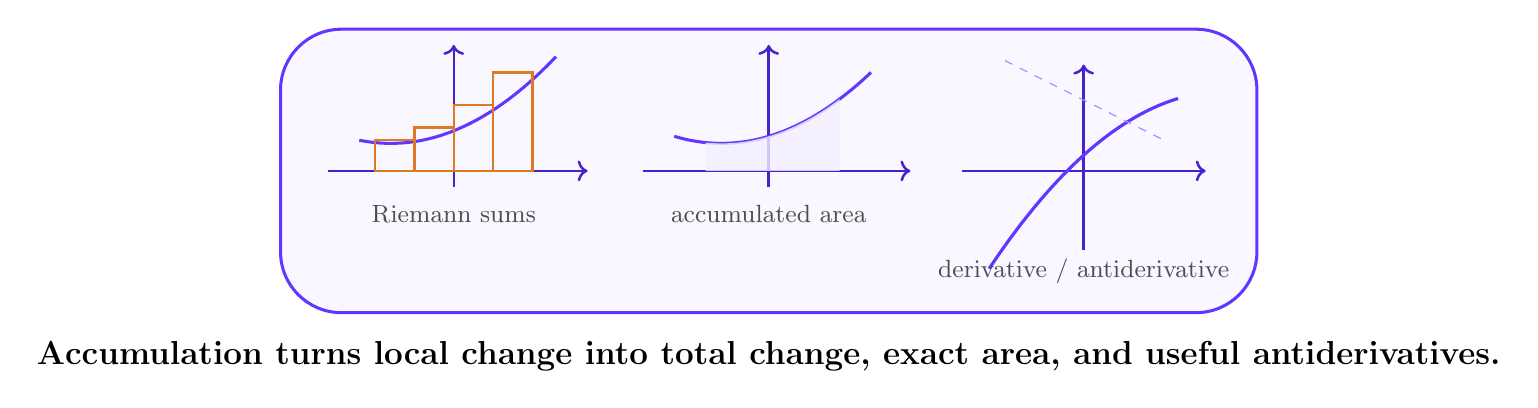
\begin{tikzpicture}[scale=1]
\fill[softlav,rounded corners=22pt] (-6.2,-1.8) rectangle (6.2,1.8);
\draw[novelPurple, line width=1.1pt, rounded corners=22pt] (-6.2,-1.8) rectangle (6.2,1.8);

% left: riemann rectangles
\begin{scope}[shift={(-4.0,0)}]
\draw[novelPurpleDark, line width=0.9pt, ->] (-1.6,0)--(1.7,0);
\draw[novelPurpleDark, line width=0.9pt, ->] (0,-0.2)--(0,1.6);
\draw[novelPurple, line width=1.1pt, smooth, domain=-1.2:1.3, samples=120]
plot (\x,{0.25*(\x+0.8)^2+0.35});
\foreach \a/\h in {-1.0/0.39,-0.5/0.55,0/0.84,0.5/1.25}{
  \draw[nporange, line width=0.9pt] (\a,0) rectangle ++(0.5,\h);
}
\node[text=npgray] at (0,-0.55) {\small Riemann sums};
\end{scope}

% middle: FTC
\begin{scope}[shift={(0,0)}]
\draw[novelPurpleDark, line width=0.9pt, ->] (-1.6,0)--(1.8,0);
\draw[novelPurpleDark, line width=0.9pt, ->] (0,-0.2)--(0,1.6);
\draw[novelPurple, line width=1.1pt, smooth, domain=-1.2:1.3, samples=120]
plot (\x,{0.25*(\x+0.6)^2+0.35});
\fill[novelPurpleLight, opacity=0.8]
(-0.8,0) -- plot[smooth, domain=-0.8:0.9, samples=100]
(\x,{0.25*(\x+0.6)^2+0.35}) -- (0.9,0) -- cycle;
\node[text=npgray] at (0,-0.55) {\small accumulated area};
\end{scope}

% right: antidifferentiation
\begin{scope}[shift={(4.0,0)}]
\draw[novelPurpleDark, line width=0.9pt, ->] (-1.55,0)--(1.55,0);
\draw[novelPurpleDark, line width=0.9pt, ->] (0,-1.0)--(0,1.35);
\draw[novelPurple, line width=1.15pt, smooth, domain=-1.2:1.2, samples=140]
plot (\x,{0.2+0.9*\x-0.25*\x*\x});
\draw[novelPurpleLine, dashed, domain=-1.0:1.0, samples=120]
plot (\x,{0.9-0.5*\x});
\node[text=npgray] at (0,-1.28) {\small derivative / antiderivative};
\end{scope}

\node[align=center] at (0,-2.35) {\large\bfseries Accumulation turns local change into total change, exact area, and useful antiderivatives.};
\end{tikzpicture}
}

\newcommand{\museumfigure}{
\begin{center}
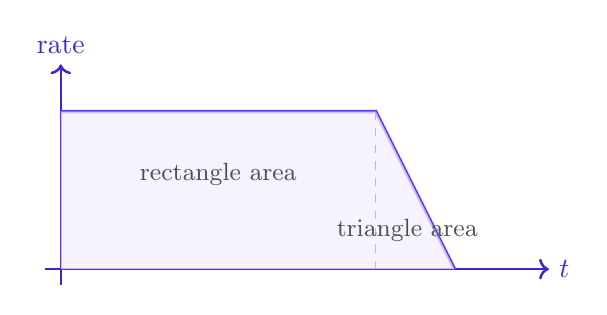
\begin{tikzpicture}[x=1cm,y=0.02cm]
\draw[novelPurpleDark, line width=0.9pt, ->] (-0.2,0)--(6.2,0) node[right] {$t$};
\draw[novelPurpleDark, line width=0.9pt, ->] (0,-10)--(0,130) node[above] {rate};

\draw[novelPurple, line width=1.2pt] (0,100)--(4,100)--(5,0);
\fill[novelPurpleLight, opacity=0.75] (0,0)--(0,100)--(4,100)--(5,0)--cycle;

\draw[gray!50, dashed] (4,0)--(4,100);
\node[text=npgray] at (2,60) {\small rectangle area};
\node[text=npgray] at (4.4,25) {\small triangle area};
\end{tikzpicture}
\end{center}
}

\newcommand{\riemannleftfigure}{
\begin{center}
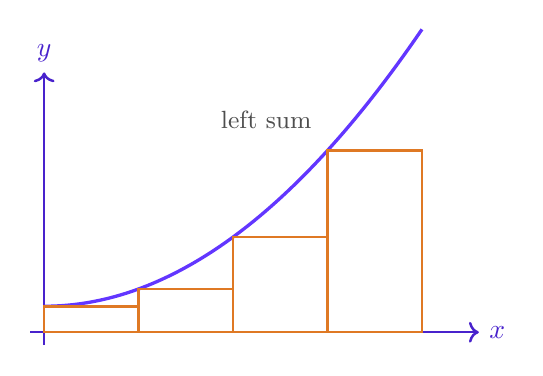
\begin{tikzpicture}[x=1.2cm,y=1.1cm]
\draw[novelPurpleDark, line width=0.9pt, ->] (-0.15,0)--(4.6,0) node[right] {$x$};
\draw[novelPurpleDark, line width=0.9pt, ->] (0,-0.15)--(0,3.0) node[above] {$y$};

\draw[novelPurple, line width=1.2pt, smooth, samples=160, domain=0:4]
plot (\x,{0.2*\x*\x+0.3});
\foreach \a/\h in {0/0.3,1/0.5,2/1.1,3/2.1}{
  \draw[nporange, line width=0.9pt] (\a,0) rectangle ++(1,\h);
}
\node[text=npgray] at (2.35,2.45) {\small left sum};
\end{tikzpicture}
\end{center}
}

\newcommand{\riemannrightfigure}{
\begin{center}
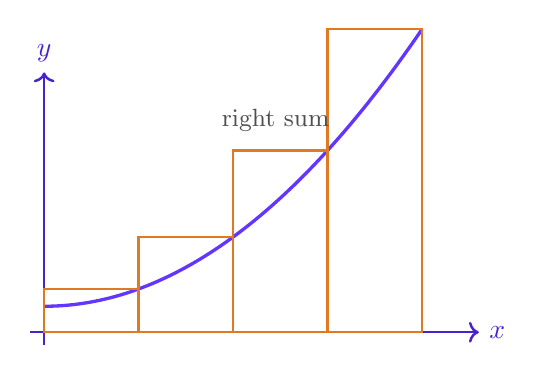
\begin{tikzpicture}[x=1.2cm,y=1.1cm]
\draw[novelPurpleDark, line width=0.9pt, ->] (-0.15,0)--(4.6,0) node[right] {$x$};
\draw[novelPurpleDark, line width=0.9pt, ->] (0,-0.15)--(0,3.0) node[above] {$y$};

\draw[novelPurple, line width=1.2pt, smooth, samples=160, domain=0:4]
plot (\x,{0.2*\x*\x+0.3});
\foreach \a/\h in {0/0.5,1/1.1,2/2.1,3/3.5}{
  \draw[nporange, line width=0.9pt] (\a,0) rectangle ++(1,\h);
}
\node[text=npgray] at (2.45,2.45) {\small right sum};
\end{tikzpicture}
\end{center}
}

\newcommand{\riemannmidfigure}{
\begin{center}
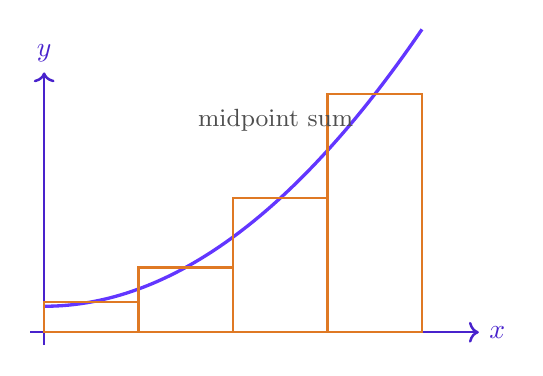
\begin{tikzpicture}[x=1.2cm,y=1.1cm]
\draw[novelPurpleDark, line width=0.9pt, ->] (-0.15,0)--(4.6,0) node[right] {$x$};
\draw[novelPurpleDark, line width=0.9pt, ->] (0,-0.15)--(0,3.0) node[above] {$y$};

\draw[novelPurple, line width=1.2pt, smooth, samples=160, domain=0:4]
plot (\x,{0.2*\x*\x+0.3});
\foreach \a/\h in {0/0.35,1/0.75,2/1.55,3/2.75}{
  \draw[nporange, line width=0.9pt] (\a,0) rectangle ++(1,\h);
}
\node[text=npgray] at (2.45,2.45) {\small midpoint sum};
\end{tikzpicture}
\end{center}
}

\newcommand{\trapezoidfigure}{
\begin{center}
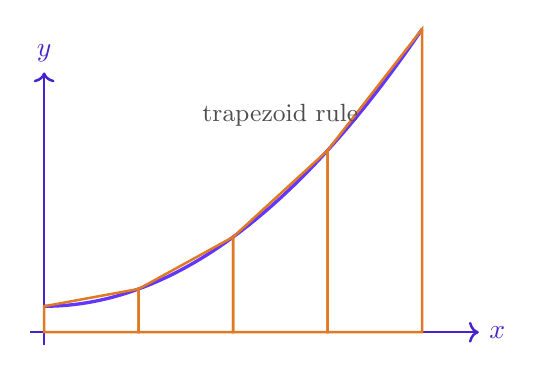
\begin{tikzpicture}[x=1.2cm,y=1.1cm]
\draw[novelPurpleDark, line width=0.9pt, ->] (-0.15,0)--(4.6,0) node[right] {$x$};
\draw[novelPurpleDark, line width=0.9pt, ->] (0,-0.15)--(0,3.0) node[above] {$y$};

\draw[novelPurple, line width=1.2pt, smooth, samples=160, domain=0:4]
plot (\x,{0.2*\x*\x+0.3});
\foreach \a/\b/\ha/\hb in {0/1/0.3/0.5,1/2/0.5/1.1,2/3/1.1/2.1,3/4/2.1/3.5}{
  \draw[nporange, line width=0.9pt] (\a,0)--(\a,\ha)--(\b,\hb)--(\b,0)--cycle;
}
\node[text=npgray] at (2.5,2.5) {\small trapezoid rule};
\end{tikzpicture}
\end{center}
}

\newcommand{\ftcaccfigure}{
\begin{center}
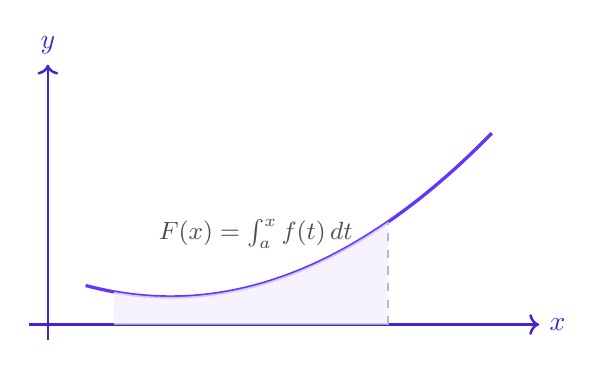
\begin{tikzpicture}[x=1.2cm,y=1cm]
\draw[novelPurpleDark, line width=0.9pt, ->] (-0.2,0)--(5.2,0) node[right] {$x$};
\draw[novelPurpleDark, line width=0.9pt, ->] (0,-0.2)--(0,3.3) node[above] {$y$};

\draw[novelPurple, line width=1.2pt, smooth, samples=140, domain=0.4:4.7]
plot (\x,{0.35 + 0.18*(\x-1.3)^2});
\fill[novelPurpleLight, opacity=0.78]
(0.7,0) -- plot[smooth, domain=0.7:3.6, samples=120]
(\x,{0.35 + 0.18*(\x-1.3)^2}) -- (3.6,0)--cycle;

\draw[gray!55, dashed] (3.6,0)--(3.6,{0.35 + 0.18*(3.6-1.3)^2});
\node[text=npgray] at (2.2,1.15) {\small \(F(x)=\int_a^x f(t)\,dt\)};
\end{tikzpicture}
\end{center}
}

\newcommand{\behaviorfigure}{
\begin{center}
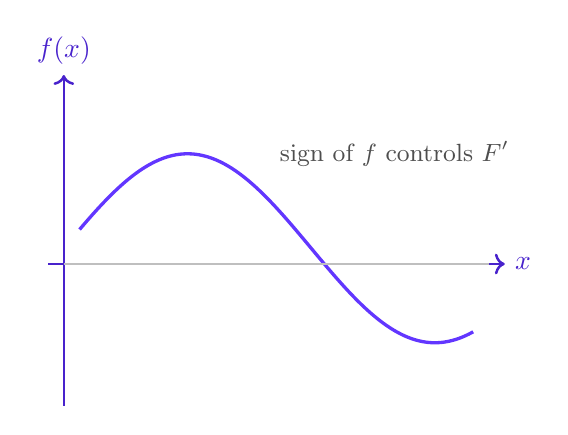
\begin{tikzpicture}[x=1.0cm,y=1.0cm]
\draw[novelPurpleDark, line width=0.9pt, ->] (-0.2,0)--(5.6,0) node[right] {$x$};
\draw[novelPurpleDark, line width=0.9pt, ->] (0,-1.8)--(0,2.4) node[above] {$f(x)$};

\draw[novelPurple, line width=1.2pt, smooth, samples=180, domain=0.2:5.2]
plot (\x,{1.2*sin(deg(\x))+0.2});
\draw[gray!50] (0,0)--(5.4,0);
\node[text=npgray] at (4.2,1.4) {\small sign of \(f\) controls \(F'\)};
\end{tikzpicture}
\end{center}
}

\newcommand{\ibpfigure}{
\begin{center}
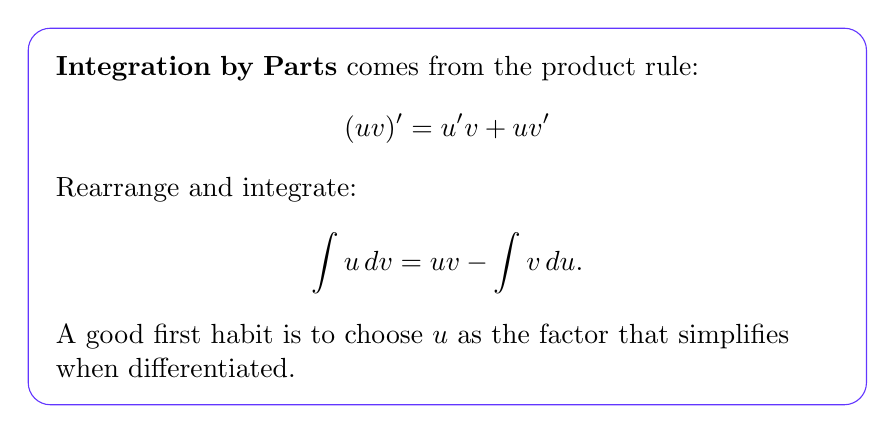
\begin{tikzpicture}[scale=1]
\node[draw=novelPurple, rounded corners=8pt, inner sep=10pt, text width=0.82\textwidth, align=left] {
\textbf{Integration by Parts} comes from the product rule:
\[
(uv)'=u'v+uv'
\]
Rearrange and integrate:
\[
\int u\,dv = uv-\int v\,du.
\]
A good first habit is to choose \(u\) as the factor that simplifies when differentiated.
};
\end{tikzpicture}
\end{center}
}

\newcommand{\techniquemap}{
\begin{center}
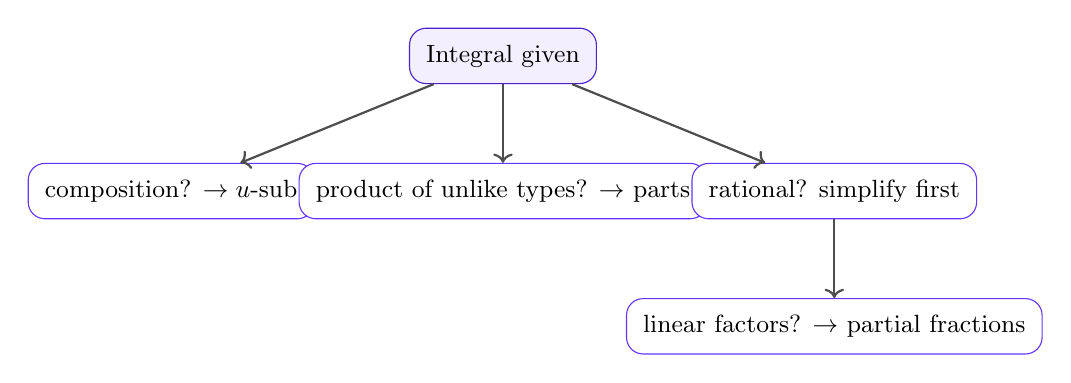
\begin{tikzpicture}[node distance=1.0cm and 1.2cm, every node/.style={font=\small}]
\node[draw=novelPurpleDark, rounded corners=6pt, fill=novelPurpleLight, inner sep=6pt] (start) {Integral given};
\node[draw=novelPurple, rounded corners=6pt, below left=of start, fill=white, inner sep=6pt] (u) {composition? \(\to u\)-sub};
\node[draw=novelPurple, rounded corners=6pt, below=of start, fill=white, inner sep=6pt] (parts) {product of unlike types? \(\to\) parts};
\node[draw=novelPurple, rounded corners=6pt, below right=of start, fill=white, inner sep=6pt] (rat) {rational? simplify first};
\node[draw=novelPurple, rounded corners=6pt, below=of rat, fill=white, inner sep=6pt] (pf) {linear factors? \(\to\) partial fractions};

\draw[->, line width=0.8pt, color=npgray] (start)--(u);
\draw[->, line width=0.8pt, color=npgray] (start)--(parts);
\draw[->, line width=0.8pt, color=npgray] (start)--(rat);
\draw[->, line width=0.8pt, color=npgray] (rat)--(pf);
\end{tikzpicture}
\end{center}
}

% =========================================================
\begin{document}

\begin{titlepage}
\centering
\vspace*{2.0cm}

{\fontsize{28}{32}\selectfont\bfseries\color{novelPurpleDark} AP Calculus AB \& BC\par}
\vspace{0.35cm}
{\fontsize{28}{32}\selectfont\bfseries\color{novelPurpleDark} Unit 6: Accumulations of Change\par}

\vspace{0.75cm}
{\Large\color{novelPurple} Optimized Novel Prep Edition\par}

\vspace{1.0cm}

\unitcoverfigure

\vfill

\begin{minipage}{0.84\textwidth}
\begin{notebox}{Design Goals for This Revision}
\begin{itemize}
    \item Keep the overall chapter sequence and mathematical scope of your original Unit 6.
    \item Upgrade the visual style to match the optimized Novel Prep Unit 7/8/9/10 system.
    \item Clarify the logic from area approximation to exact accumulation and antiderivatives.
    \item Preserve the original example path whenever possible while fixing wording, notation, and setup issues.
    \item Make the chapter useful for both first instruction and AP review.
\end{itemize}
\end{notebox}
\end{minipage}

\vfill

{\large\textbf{Novel Prep Learning Center}}\\[0.25em]
{\large J. Z}

\end{titlepage}

\tableofcontents
\newpage

\setcounter{section}{5}
\section{Accumulations of Change}

\begin{theorybox}{Big Idea}
Unit 6 is where students first see integration as more than an operation.  
It becomes:
\[
\text{area} \longrightarrow \text{net change} \longrightarrow \text{accumulation} \longrightarrow \text{antiderivative}.
\]
This chapter connects geometric reasoning, sigma notation, exact integrals, and techniques of antidifferentiation.
\end{theorybox}

\begin{notebox}{Teaching Philosophy for This Unit}
Students should not memorize integration as a list of formulas.  
They should understand that the same central idea keeps reappearing:

\[
\textit{Many tiny pieces of change can be added to produce a meaningful total.}
\]

That idea appears numerically, graphically, analytically, and verbally throughout the unit.
\end{notebox}

\apcheckpoint{
The chapter naturally unfolds in four layers:
\begin{itemize}
    \item \textbf{Approximation:} Riemann sums and numerical area.
    \item \textbf{Exact accumulation:} definite integrals and FTC.
    \item \textbf{Reverse differentiation:} antiderivatives and indefinite integrals.
    \item \textbf{Technique selection:} substitution, parts, partial fractions, and improper integrals.
\end{itemize}
}

% =========================================================
\unitchapter{Exploring Accumulations of Change}

\begin{theorybox}{Definition 6.1.1 --- Accumulations of Change}
The accumulation of change is the total amount of change in a quantity over a given interval.  
It can often be computed by:
\begin{itemize}
    \item integrating a rate function, or
    \item finding the signed area under a rate-of-change graph.
\end{itemize}
\end{theorybox}

\museumfigure

\example{Museum attendance accumulation}
The graph shows the rate of change for the number of people in a museum \(t\) hours after it opens.  
How many people have entered the museum after \(5\) hours?

\solution
We compute the total accumulated change by area.

From \(t=0\) to \(t=4\), the graph is a rectangle of height \(100\):
\[
100\cdot 4=400.
\]
From \(t=4\) to \(t=5\), the graph forms a triangle of base \(1\) and height \(100\):
\[
\frac12(1)(100)=50.
\]
Thus the total number of people is
\[
\boxed{450.}
\]

\example{A second accumulation example}
Water flows into a tank at a rate of \(r(t)\) gallons per minute. Explain what
\[
\int_0^6 r(t)\,dt
\]
represents.

\solution
This integral represents the total amount of water added to the tank during the first \(6\) minutes.

% =========================================================
\unitchapter{Approximating Area with Riemann Sums}

\begin{notebox}{Approximation of Area with Riemann Sums}
To approximate the area under a curve:
\begin{enumerate}
    \item divide the interval into smaller subintervals,
    \item choose a sample point in each subinterval,
    \item build rectangles using those heights,
    \item and add the rectangle areas.
\end{enumerate}
\end{notebox}

\unitsubtopic{Left Riemann Sum}

\begin{theorybox}{Theorem 6.2.1 --- Left Riemann Sum}
For equal subinterval width \(\Delta x\), the left Riemann sum is
\[
A_{\text{left}}=\Delta x\big[f(x_0)+f(x_1)+\cdots+f(x_{n-1})\big].
\]
\end{theorybox}

\riemannleftfigure

\example{Left Riemann sum}
Given
\[
f(x)=\frac12x^3-x^2+x+2,
\]
compute the left Riemann sum on \([1,3]\) with \(4\) subintervals.

\solution
\[
\Delta x=\frac{3-1}{4}=\frac12.
\]
Left endpoints:
\[
x_0=1,\quad x_1=1.5,\quad x_2=2,\quad x_3=2.5.
\]
Function values:
\[
f(1)=2.5,\quad f(1.5)=2.9375,\quad f(2)=4,\quad f(2.5)=6.0625.
\]
So
\[
A_{\text{left}}=\frac12(2.5+2.9375+4+6.0625)=\frac12(15.5)=\boxed{7.75}.
\]

\unitsubtopic{Right Riemann Sum}

\begin{theorybox}{Theorem 6.2.2 --- Right Riemann Sum}
For equal subinterval width \(\Delta x\), the right Riemann sum is
\[
A_{\text{right}}=\Delta x\big[f(x_1)+f(x_2)+\cdots+f(x_n)\big].
\]
\end{theorybox}

\riemannrightfigure

\example{Right Riemann sum}
Given
\[
f(x)=\sqrt{9-x^2},
\]
compute the right Riemann sum on \([-2,1]\) with \(3\) subintervals.

\solution
\[
\Delta x=\frac{1-(-2)}{3}=1.
\]
Right endpoints:
\[
x_1=-1,\quad x_2=0,\quad x_3=1.
\]
Then
\[
f(-1)=\sqrt8,\qquad f(0)=3,\qquad f(1)=\sqrt8.
\]
Thus
\[
A_{\text{right}}=1(\sqrt8+3+\sqrt8)=3+2\sqrt8\approx \boxed{8.6568}.
\]

\unitsubtopic{Midpoint Riemann Sum}

\begin{theorybox}{Theorem 6.2.3 --- Midpoint Riemann Sum}
For equal subinterval width \(\Delta x\), the midpoint Riemann sum is
\[
A_{\text{mid}}=\Delta x\sum_{i=1}^{n} f\!\left(\frac{x_{i-1}+x_i}{2}\right).
\]
\end{theorybox}

\riemannmidfigure

\example{Midpoint rule with tabular data}
A rectangular pool gets deeper from one end to the other. The table shows the depth \(h(x)\) of the water at \(4\)-foot intervals:

\[
\begin{array}{c|ccccccc}
x(\text{ft}) & 0 & 4 & 8 & 12 & 16 & 20 & 24\\
\hline
h(x)(\text{ft}) & 6.5 & 8 & 9.5 & 10 & 11 & 11.5 & 12
\end{array}
\]

Use a midpoint Riemann sum with \(\Delta x=8\) on the intervals \([0,8],[8,16],[16,24]\).

\solution
The three subintervals have midpoints
\[
x=4,\quad x=12,\quad x=20.
\]
So
\[
A\approx 8\,[h(4)+h(12)+h(20)]
=8(8+10+11.5)=8(29.5)=\boxed{236}.
\]
\newpage
\unitsubtopic{Trapezoid Rule}

\begin{theorybox}{Theorem 6.2.4 --- Trapezoid Rule}
For equal subinterval width \(\Delta x\),
\[
T_n=\frac{\Delta x}{2}\Big[f(x_0)+2f(x_1)+2f(x_2)+\cdots+2f(x_{n-1})+f(x_n)\Big].
\]
\end{theorybox}

\trapezoidfigure

\example{Trapezoidal approximation with unequal widths}
The rate at which customers are being served is given by the table:

\[
\begin{array}{c|ccccc}
t(\text{hours}) & 0 & 2 & 3 & 6 & 10\\
\hline
R(t)(\text{people/hour}) & 37 & 44 & 36 & 42 & 48
\end{array}
\]

At \(t=0\), \(200\) customers had already been served. Use trapezoids to approximate the total number served after \(10\) hours.

\solution
Because the widths are not equal, compute each trapezoid separately:
\[
2\cdot \frac{37+44}{2}
+1\cdot \frac{44+36}{2}
+3\cdot \frac{36+42}{2}
+4\cdot \frac{42+48}{2}.
\]
This gives
\[
81+40+117+180=418.
\]
Including the initial \(200\) customers:
\[
200+418=\boxed{618}.
\]

% =========================================================
\unitchapter{Riemann Sums, Summation Notation, and Definite Integral Notation}

\unitsubtopic{Sigma Notation}

\begin{theorybox}{Definition 6.3.1 --- Sigma Notation}
The sum of terms
\[
a_1+a_2+\cdots+a_n
\]
can be written as
\[
\sum_{i=1}^n a_i.
\]
\end{theorybox}

\begin{theorybox}{Theorem 6.3.1 --- Summation Formulas}
\[
\sum_{i=1}^n c=cn,\qquad
\sum_{i=1}^n i=\frac{n(n+1)}{2},
\]
\[
\sum_{i=1}^n i^2=\frac{n(n+1)(2n+1)}{6},\qquad
\sum_{i=1}^n i^3=\frac{n^2(n+1)^2}{4}.
\]
\end{theorybox}

\example{Examples of sigma notation}
Rewrite the following in expanded form:

\begin{enumerate}[label=\textbf{(\alph*)}]
    \item \(\displaystyle \sum_{i=1}^6 i\)
    \item \(\displaystyle \sum_{j=3}^7 j^2\)
    \item \(\displaystyle \sum_{i=1}^n f(x_i)\Delta x\)
\end{enumerate}

\solution
\begin{enumerate}[label=\textbf{(\alph*)}]
    \item
    \[
    1+2+3+4+5+6
    \]
    \item
    \[
    3^2+4^2+5^2+6^2+7^2
    \]
    \item
    \[
    f(x_1)\Delta x+f(x_2)\Delta x+\cdots+f(x_n)\Delta x
    \]
\end{enumerate}

\example{Evaluating a sum}
Evaluate
\[
\sum_{i=1}^{n}\frac{i+1}{n^2}.
\]

\solution
\[
\sum_{i=1}^{n}\frac{i+1}{n^2}
=
\frac{1}{n^2}\sum_{i=1}^{n}(i+1)
=
\frac{1}{n^2}\left(\sum_{i=1}^{n}i+\sum_{i=1}^{n}1\right).
\]
So
\[
=
\frac{1}{n^2}\left(\frac{n(n+1)}{2}+n\right)
=
\frac{1}{n^2}\cdot \frac{n^2+3n}{2}
=
\boxed{\frac{n+3}{2n}}.
\]

\unitsubtopic{Riemann Sums}

\begin{theorybox}{Definition 6.3.2 --- Riemann Sum}
Let \([a,b]\) be partitioned into subintervals and let \(c_i\) be a sample point in the \(i\)-th subinterval. Then
\[
\sum_{i=1}^{n} f(c_i)\Delta x_i
\]
is a Riemann sum for \(f\).
\end{theorybox}

\example{Riemann sum in summation notation}
Find the right Riemann sum with \(4\) subdivisions for
\[
f(x)=e^x
\]
on \([1,3]\).

\solution
\[
\Delta x=\frac{3-1}{4}=0.5.
\]
Right endpoints:
\[
1.5,\ 2.0,\ 2.5,\ 3.0.
\]
Thus
\[
A_{\text{right}}=\sum_{i=1}^{4} f(x_i)\Delta x
=
0.5\,[e^{1.5}+e^{2}+e^{2.5}+e^{3}].
\]

\begin{theorybox}{Theorem 6.3.2 --- Limits of Lower and Upper Sums}
If \(f\) is continuous and nonnegative on \([a,b]\), then the lower and upper sums both approach the same limit as the partition gets finer. That common limit is the exact area.
\end{theorybox}

\example{Area by the limit definition}
Find the area under
\[
f(x)=x^3
\]
from \(x=0\) to \(x=1\) using the limit definition.

\solution
Take
\[
\Delta x=\frac{1}{n},\qquad c_i=\frac{i}{n}.
\]
Then
\[
A=\lim_{n\to\infty}\sum_{i=1}^{n}f(c_i)\Delta x
=
\lim_{n\to\infty}\sum_{i=1}^{n}\left(\frac{i}{n}\right)^3\frac{1}{n}
=
\lim_{n\to\infty}\frac{1}{n^4}\sum_{i=1}^{n}i^3.
\]
Use the sum formula:
\[
=
\lim_{n\to\infty}\frac{1}{n^4}\cdot \frac{n^2(n+1)^2}{4}
=
\lim_{n\to\infty}\frac{(n+1)^2}{4n^2}
=
\boxed{\frac14}.
\]

\unitsubtopic{Definite Integrals}

\begin{theorybox}{Definition 6.3.3 --- Definite Integral}
If the limit of Riemann sums exists, then
\[
\int_a^b f(x)\,dx
\]
denotes that limit and is called the definite integral of \(f\) from \(a\) to \(b\).
\end{theorybox}

\begin{theorybox}{Theorem 6.3.3 --- Continuity Implies Integrability}
If \(f\) is continuous on \([a,b]\), then \(f\) is integrable on \([a,b]\).
\end{theorybox}

\example{Evaluating a definite integral as a limit}
Evaluate
\[
\int_{-2}^{1} 2x\,dx
\]
using the limit definition.

\solution
\[
\Delta x=\frac{1-(-2)}{n}=\frac{3}{n}.
\]
Choose right endpoints:
\[
c_i=-2+\frac{3i}{n}.
\]
Then
\[
\int_{-2}^{1}2x\,dx
=
\lim_{n\to\infty}\sum_{i=1}^{n}2\left(-2+\frac{3i}{n}\right)\frac{3}{n}.
\]
Simplifying the sum leads to
\[
\boxed{-3}.
\]

% =========================================================
\unitchapter{The Fundamental Theorem of Calculus and Accumulation Functions (Derivative Part)}

\begin{theorybox}{Theorem 6.4.1 --- FTC, Derivative Part}
If \(f\) is continuous and
\[
F(x)=\int_a^x f(t)\,dt,
\]
then
\[
F'(x)=f(x).
\]
\end{theorybox}

\ftcaccfigure

\example{Basic FTC derivative}
Evaluate
\[
\frac{d}{dx}\left[\int_0^x \sqrt{t^2+1}\,dt\right].
\]

\solution
By the Fundamental Theorem of Calculus,
\[
\frac{d}{dx}\left[\int_0^x \sqrt{t^2+1}\,dt\right]
=
\boxed{\sqrt{x^2+1}}.
\]

\begin{notebox}{Lower Limit of Integration}
If the variable appears as the lower limit, reverse the limits first:
\[
\frac{d}{dx}\int_x^3 f(t)\,dt
=
-\frac{d}{dx}\int_3^x f(t)\,dt
=
-f(x).
\]
\end{notebox}

\begin{notebox}{More Complicated Functions in the Limit}
If the upper limit is \(h(x)\), then
\[
\frac{d}{dx}\int_a^{h(x)} f(t)\,dt=f(h(x))h'(x).
\]
This is FTC plus the chain rule.
\end{notebox}

\example{FTC with chain rule}
If
\[
F(x)=\int_{\pi/2}^{x^3}\cos t\,dt,
\]
find \(F'(x)\).

\solution
\[
F'(x)=\cos(x^3)\cdot 3x^2.
\]
So
\[
\boxed{F'(x)=3x^2\cos(x^3).}
\]

\example{Variable limits on both sides}
Let
\[
h(x)=\int_{3x^2}^{x^3}\sqrt{16-t^2}\,dt.
\]
Find \(h'(1)\).

\solution
\[
h'(x)=\sqrt{16-(x^3)^2}\cdot 3x^2-\sqrt{16-(3x^2)^2}\cdot 6x.
\]
Evaluate at \(x=1\):
\[
h'(1)=3\sqrt{15}-6\sqrt7.
\]
Thus
\[
\boxed{h'(1)=3\sqrt{15}-6\sqrt7.}
\]

% =========================================================
\unitchapter{Behavior of Accumulation Functions Involving Area}

\begin{notebox}{Key Idea}
If
\[
F(x)=\int_a^x f(t)\,dt,
\]
then
\[
F'(x)=f(x).
\]
So the sign and behavior of \(f\) determine the increasing/decreasing behavior of \(F\).
\end{notebox}

\behaviorfigure

\example{Using \(f\) to analyze \(F\)}
Suppose
\[
F(x)=\int_a^x f(t)\,dt.
\]
Explain how to determine where \(F\) is increasing.

\solution
Since
\[
F'(x)=f(x),
\]
the function \(F\) is increasing whenever
\[
f(x)>0.
\]

\example{Local extrema of accumulation functions}
When does \(F(x)=\int_a^x f(t)\,dt\) have a local maximum or minimum?

\solution
Local extrema occur where \(F'(x)=f(x)=0\) and the sign of \(f\) changes.

% =========================================================
\unitchapter{Properties of Definite Integrals}

\begin{theorybox}{Properties of Definite Integrals}
For integrable functions \(f\) and \(g\) and constant \(c\):
\[
\int_a^a f(x)\,dx=0,
\]
\[
\int_a^b f(x)\,dx=-\int_b^a f(x)\,dx,
\]
\[
\int_a^b cf(x)\,dx=c\int_a^b f(x)\,dx,
\]
\[
\int_a^b \big(f(x)\pm g(x)\big)\,dx=\int_a^b f(x)\,dx\pm \int_a^b g(x)\,dx,
\]
\[
\int_a^c f(x)\,dx+\int_c^b f(x)\,dx=\int_a^b f(x)\,dx.
\]
\end{theorybox}

\example{Basic integral properties}
If
\[
\int_7^2 f(x)\,dx=-5,
\]
find
\[
\int_2^7 f(x)\,dx.
\]

\solution
Reverse the limits:
\[
\int_2^7 f(x)\,dx=-\int_7^2 f(x)\,dx=5.
\]

\example{Using area from a graph}
Suppose a graph provides the following values:
\[
\int_{-4}^{-1} f(x)\,dx=3,\qquad
\int_1^2 f(x)\,dx=-1.5,\qquad
\int_1^5 2f(x)\,dx=18.
\]
Evaluate each quantity using integral properties.

\solution
Use linearity, sign reversal, and interval additivity exactly as needed.  
This is the kind of section where students should practice \emph{reasoning from known values}, not recomputing from scratch.

\example{Additive interval property}
If
\[
\int_1^5 f(x)\,dx=3,\qquad
\int_5^{10} f(x)\,dx=5,\qquad
\int_{10}^{13} f(x)\,dx=-7,
\]
find
\[
\int_1^{13} f(x)\,dx.
\]

\solution
\[
\int_1^{13} f(x)\,dx
=
\int_1^5 f(x)\,dx+\int_5^{10} f(x)\,dx+\int_{10}^{13} f(x)\,dx
=3+5-7=\boxed{1}.
\]

% =========================================================
\unitchapter{The Fundamental Theorem of Calculus and Definite Integrals}

\unitsubtopic{Fundamental Theorem of Calculus Part 1}

\begin{theorybox}{Theorem 6.7.1 --- FTC Part 1}
If
\[
g(x)=\int_a^x f(t)\,dt,
\]
then
\[
g'(x)=f(x).
\]
\end{theorybox}

\unitsubtopic{Fundamental Theorem of Calculus Part 2}

\begin{theorybox}{Theorem 6.7.2 --- FTC Part 2}
If \(f\) is continuous on \([a,b]\) and \(F\) is an antiderivative of \(f\), then
\[
\int_a^b f(x)\,dx=F(b)-F(a).
\]
\end{theorybox}

\example{Evaluating a definite integral with an antiderivative}
Evaluate
\[
\int_1^4 (3x^2-2x)\,dx.
\]

\solution
An antiderivative is
\[
F(x)=x^3-x^2.
\]
So
\[
\int_1^4 (3x^2-2x)\,dx
=
F(4)-F(1)
=
(64-16)-(1-1)=\boxed{48}.
\]

\example{Graph interpretation with FTC}
If
\[
\int_3^0 f(x)\,dx=3.5
\]
and \(F'(x)=f(x)\), explain how to find \(F(4)-F(0)\).

\solution
Use
\[
F(4)-F(0)=\int_0^4 f(x)\,dx
\]
and break the interval into known parts.

% =========================================================
\unitchapter{Finding Antiderivatives and Indefinite Integrals}

\unitsubtopic{The Antiderivative of a Function}

\begin{theorybox}{Definition 6.8.1 --- Antiderivative}
A function \(F\) is an antiderivative of \(f\) on an interval if
\[
F'(x)=f(x)
\]
for all \(x\) in the interval.
\end{theorybox}

\begin{theorybox}{Definition 6.8.2 --- Indefinite Integral}
The indefinite integral of \(f\) is the family of all antiderivatives of \(f\):
\[
\int f(x)\,dx=F(x)+C.
\]
\end{theorybox}

\unitsubtopic{Antidifferentiation Formulas}

\begin{theorybox}{Core Antidifferentiation Formulas}
\[
\int x^n\,dx=\frac{x^{n+1}}{n+1}+C \qquad (n\neq -1)
\]
\[
\int \frac{1}{x}\,dx=\ln|x|+C
\]
\[
\int e^x\,dx=e^x+C,\qquad \int a^x\,dx=\frac{a^x}{\ln a}+C
\]
\[
\int \sin x\,dx=-\cos x+C,\qquad \int \cos x\,dx=\sin x+C
\]
\[
\int \sec^2x\,dx=\tan x+C,\qquad \int \frac{1}{1+x^2}\,dx=\tan^{-1}x+C
\]
\end{theorybox}

\example{Finding an antiderivative}
Find \(g(x)\) if
\[
g'(x)=4\sin x+2x^4-x^{-1/2}.
\]

\solution
\[
g(x)=4(-\cos x)+2\cdot\frac{x^5}{5}-\frac{x^{1/2}}{1/2}+C
=
\boxed{-4\cos x+\frac{2}{5}x^5-2\sqrt{x}+C.}
\]

\example{Antiderivative with an initial condition}
Find \(f\) if
\[
f'(x)=e^x+20(1+x^2)^{-1}
\]
and \(f(0)=-2\).

\solution
\[
f(x)=e^x+20\tan^{-1}x+C.
\]
Use \(f(0)=-2\):
\[
1+0+C=-2 \Rightarrow C=-3.
\]
So
\[
\boxed{f(x)=e^x+20\tan^{-1}x-3.}
\]

\example{Second derivative data}
Find \(f\) if
\[
f''(x)=12x^2+6x-4,\qquad f(0)=4,\qquad f(1)=1.
\]

\solution
Integrate once:
\[
f'(x)=4x^3+3x^2-4x+C.
\]
Integrate again:
\[
f(x)=x^4+x^3-2x^2+Cx+D.
\]
Use \(f(0)=4\) to get \(D=4\).  
Use \(f(1)=1\):
\[
1+1-2+C+4=1 \Rightarrow C=-3.
\]
Thus
\[
\boxed{f(x)=x^4+x^3-2x^2-3x+4.}
\]

% =========================================================
\unitchapter{Integrating Using Substitution}

\unitsubtopic{Substitution: Indefinite Integrals}

\begin{theorybox}{Substitution Rule}
If \(u=g(x)\), then
\[
\int f(g(x))g'(x)\,dx=\int f(u)\,du.
\]
\end{theorybox}

\example{Basic \(u\)-substitution}
Evaluate
\[
\int 2x(x^2+1)^5\,dx.
\]

\solution
Let
\[
u=x^2+1,\qquad du=2x\,dx.
\]
Then
\[
\int 2x(x^2+1)^5\,dx=\int u^5\,du=\frac{u^6}{6}+C
=\boxed{\frac{(x^2+1)^6}{6}+C.}
\]

\example{Trigonometric substitution-style \(u\)-sub}
Evaluate
\[
\int \sin(3x)\,dx.
\]

\solution
Let \(u=3x\), so \(du=3dx\) and \(dx=\frac13du\). Then
\[
\int \sin(3x)\,dx=\frac13\int \sin u\,du
=
-\frac13\cos u+C
=
\boxed{-\frac13\cos(3x)+C.}
\]

\unitsubtopic{Substitution: Definite Integrals}

\example{Definite integral with substitution}
Evaluate
\[
\int_0^1 2x(x^2+1)^3\,dx.
\]

\solution
Let \(u=x^2+1\), so \(du=2x\,dx\). Change limits:
\[
x=0 \Rightarrow u=1,\qquad x=1 \Rightarrow u=2.
\]
Then
\[
\int_0^1 2x(x^2+1)^3\,dx=\int_1^2 u^3\,du
=\left[\frac{u^4}{4}\right]_1^2
=
\frac{16-1}{4}
=
\boxed{\frac{15}{4}.}
\]

% =========================================================
\unitchapter{Integrating Functions Using Long Division and Completing the Square}

\unitsubtopic{Integrating Using Long Division}

\example{Long division first}
Evaluate
\[
\int \frac{x^2+3x+1}{x+1}\,dx.
\]

\solution
Divide:
\[
\frac{x^2+3x+1}{x+1}=x+2-\frac{1}{x+1}.
\]
So
\[
\int \frac{x^2+3x+1}{x+1}\,dx
=
\int \left(x+2-\frac{1}{x+1}\right)\,dx
=
\boxed{\frac{x^2}{2}+2x-\ln|x+1|+C.}
\]

\unitsubtopic{Integrating Using Complete the Square}

\example{Complete the square}
Evaluate
\[
\int \frac{1}{x^2+4x+13}\,dx.
\]

\solution
Complete the square:
\[
x^2+4x+13=(x+2)^2+9.
\]
Thus
\[
\int \frac{1}{(x+2)^2+3^2}\,dx
=
\frac13\tan^{-1}\left(\frac{x+2}{3}\right)+C.
\]
So
\[
\boxed{\int \frac{1}{x^2+4x+13}\,dx
=
\frac13\tan^{-1}\left(\frac{x+2}{3}\right)+C.}
\]

% =========================================================
\unitchapter{Integrating Using Integration by Parts}

\begin{theorybox}{Theorem 6.11.1 --- Integration by Parts}
\[
\int u\,dv=uv-\int v\,du.
\]
\end{theorybox}

\ibpfigure

\example{Basic integration by parts}
Evaluate
\[
\int x e^x\,dx.
\]

\solution
Choose
\[
u=x,\qquad dv=e^x\,dx.
\]
Then
\[
du=dx,\qquad v=e^x.
\]
So
\[
\int xe^x\,dx=xe^x-\int e^x\,dx=xe^x-e^x+C.
\]
Thus
\[
\boxed{\int xe^x\,dx=e^x(x-1)+C.}
\]

\example{Logarithm example}
Evaluate
\[
\int \ln x\,dx.
\]

\solution
Write
\[
\int \ln x\,dx=\int (\ln x)(1)\,dx.
\]
Choose
\[
u=\ln x,\qquad dv=dx.
\]
Then
\[
du=\frac{1}{x}dx,\qquad v=x.
\]
So
\[
\int \ln x\,dx=x\ln x-\int 1\,dx=x\ln x-x+C.
\]
Hence
\[
\boxed{\int \ln x\,dx=x\ln x-x+C.}
\]

% =========================================================
\unitchapter{Integrating Using Linear Partial Fractions}

\begin{theorybox}{Linear Partial Fractions}
If a rational function has distinct linear factors in the denominator, rewrite it as a sum of simpler fractions before integrating.
\end{theorybox}

\example{Basic partial fractions}
Evaluate
\[
\int \frac{1}{x^2-x-2}\,dx.
\]

\solution
Factor:
\[
x^2-x-2=(x-2)(x+1).
\]
Write
\[
\frac{1}{(x-2)(x+1)}=\frac{A}{x-2}+\frac{B}{x+1}.
\]
Solving gives
\[
A=\frac13,\qquad B=-\frac13.
\]
So
\[
\int \frac{1}{x^2-x-2}\,dx
=
\frac13\int \frac{1}{x-2}\,dx-\frac13\int \frac{1}{x+1}\,dx.
\]
Thus
\[
\boxed{\int \frac{1}{x^2-x-2}\,dx
=
\frac13\ln|x-2|-\frac13\ln|x+1|+C.}
\]

% =========================================================
\unitchapter{Evaluating Improper Integrals}

\unitsubtopic{Improper Integrals with Infinite Limits of Integration}

\begin{theorybox}{Definition 6.13.1 --- Infinite Limits}
If an upper limit is infinite, define
\[
\int_a^{\infty} f(x)\,dx
=
\lim_{b\to\infty}\int_a^b f(x)\,dx.
\]
\end{theorybox}

\example{Infinite upper limit}
Evaluate
\[
\int_1^\infty \frac{1}{x^2}\,dx.
\]

\solution
\[
\int_1^\infty \frac{1}{x^2}\,dx
=
\lim_{b\to\infty}\int_1^b x^{-2}\,dx
=
\lim_{b\to\infty}\left[-\frac{1}{x}\right]_1^b
=
\lim_{b\to\infty}\left(-\frac{1}{b}+1\right)
=
\boxed{1.}
\]

\unitsubtopic{Improper Integrals with Infinite Discontinuities}

\begin{theorybox}{Definition 6.13.2 --- Infinite Discontinuities}
If \(f\) has an infinite discontinuity at \(x=c\), then the integral is defined as a limit approaching \(c\).
\end{theorybox}

\example{Improper integral with a vertical asymptote}
Evaluate
\[
\int_0^1 \frac{1}{\sqrt{x}}\,dx.
\]

\solution
\[
\int_0^1 \frac{1}{\sqrt{x}}\,dx
=
\lim_{a\to 0^+}\int_a^1 x^{-1/2}\,dx
=
\lim_{a\to 0^+}\left[2\sqrt{x}\right]_a^1
=
\lim_{a\to 0^+}(2-2\sqrt{a})
=
\boxed{2.}
\]

% =========================================================
\unitchapter{Selecting Techniques for Antidifferentiation}

\begin{theorybox}{Technique Selection}
When choosing an integration method, ask:
\begin{itemize}
    \item Is it already a basic antiderivative?
    \item Is there an obvious inner function? \(\to\) substitution
    \item Is it a product of unlike types? \(\to\) parts
    \item Is it a rational function? \(\to\) simplify first
    \item Is the rational denominator factorable? \(\to\) partial fractions
\end{itemize}
\end{theorybox}

\techniquemap

\example{Choosing a technique}
Which technique is most appropriate for each integral?

\begin{enumerate}[label=\textbf{(\alph*)}]
    \item \(\displaystyle \int x e^x\,dx\)
    \item \(\displaystyle \int \frac{2x}{x^2+5}\,dx\)
    \item \(\displaystyle \int \frac{x^2+1}{x+1}\,dx\)
    \item \(\displaystyle \int \frac{1}{(x-1)(x+2)}\,dx\)
\end{enumerate}

\solution
\begin{enumerate}[label=\textbf{(\alph*)}]
    \item integration by parts
    \item substitution
    \item long division first
    \item partial fractions
\end{enumerate}

% =========================================================
\newpage
\subsection{Unit 6 Summary / Formula Sheet}

\begin{summarybox}{Unit 6 Master Summary Sheet}
\renewcommand{\arraystretch}{1.35}
\begin{tabularx}{\textwidth}{@{}p{0.37\textwidth}X@{}}
\toprule
\textbf{Topic} & \textbf{Key Formula / Idea} \\
\midrule
Left Riemann sum & \(\Delta x[f(x_0)+\cdots+f(x_{n-1})]\) \\

Right Riemann sum & \(\Delta x[f(x_1)+\cdots+f(x_n)]\) \\

Midpoint sum & \(\Delta x\sum f\!\left(\frac{x_{i-1}+x_i}{2}\right)\) \\

Trapezoid rule & \(\frac{\Delta x}{2}[f(x_0)+2f(x_1)+\cdots+f(x_n)]\) for equal widths \\

Definite integral & limit of Riemann sums \\

FTC derivative part & \(\frac{d}{dx}\int_a^x f(t)\,dt=f(x)\) \\

FTC evaluation part & \(\int_a^b f(x)\,dx=F(b)-F(a)\) \\

Indefinite integral & \(\int f(x)\,dx=F(x)+C\) \\

Substitution & match inner function and derivative \\

Integration by parts & \(\int u\,dv=uv-\int v\,du\) \\

Partial fractions & split rational expressions after factoring \\

Improper integrals & evaluate as limits \\
\bottomrule
\end{tabularx}
\end{summarybox}

\vspace{1em}

\begin{summarybox}{Strategy Ladder}
\begin{itemize}
    \item Start with approximation when exact area is hard.
    \item Move from rectangles to the definite integral as a limit.
    \item Use FTC to connect area and derivatives.
    \item Think of antiderivatives as reversing derivatives.
    \item Choose the simplest valid technique before using a more advanced one.
\end{itemize}
\end{summarybox}

% =========================================================
\newpage
\subsection{Guided Practice Set}

\begin{practicebox}{Guided Practice A --- Approximation and Riemann Sums}
\begin{enumerate}
    \item Compute a left Riemann sum for \(f(x)=x^2\) on \([0,2]\) with \(4\) equal subintervals.
    \item Compute a midpoint sum for the same function and interval.
    \item Explain when a left sum underestimates the area.
    \item Explain why trapezoid rule is often more accurate than left or right sums.
\end{enumerate}
\end{practicebox}

\begin{practicebox}{Guided Practice B --- FTC and Definite Integrals}
\begin{enumerate}
    \item Evaluate \(\frac{d}{dx}\int_0^x (t^2+1)\,dt\).
    \item Evaluate \(\frac{d}{dx}\int_1^{x^2}\sin t\,dt\).
    \item Evaluate \(\int_1^3 2x\,dx\).
    \item Explain the difference between \(\int_a^x f(t)\,dt\) and \(\int_a^b f(x)\,dx\).
\end{enumerate}
\end{practicebox}

\begin{practicebox}{Guided Practice C --- Antidifferentiation Techniques}
\begin{enumerate}
    \item Find \(\int (3x^2-4)\,dx\).
    \item Find \(\int 2x(x^2+1)^4\,dx\).
    \item Find \(\int xe^x\,dx\).
    \item Decide which technique should be used for \(\int \frac{x^2+1}{x-1}\,dx\).
\end{enumerate}
\end{practicebox}

% =========================================================
\newpage
\subsection{Homework / Class Exercises}

\begin{homeworkset}{Level 1 --- Skill Check}
\begin{enumerate}
    \item Find a left Riemann sum for \(f(x)=x+1\) on \([0,3]\) with \(3\) equal subintervals.
    \hwspace

    \item Find a right Riemann sum for \(f(x)=x+1\) on \([0,3]\) with \(3\) equal subintervals.
    \hwspace

    \item Evaluate \(\int_0^2 (3x^2+1)\,dx\).
    \hwspace

    \item Evaluate \(\dfrac{d}{dx}\left[\int_1^x \sqrt{t+4}\,dt\right]\).
    \hwspace

    \item Find \(\int (x^3-2x+5)\,dx\).
\end{enumerate}
\end{homeworkset}

\begin{homeworkset}{Level 2 --- AP Style Practice}
\begin{enumerate}
\setcounter{enumi}{5}
    \item Use the limit definition to evaluate \(\int_0^1 x\,dx\).
    \hwspace

    \item If \(F(x)=\int_2^{x^3}\cos t\,dt\), find \(F'(x)\).
    \hwspace

    \item Find \(\int 2x(x^2+5)^3\,dx\).
    \hwspace

    \item Find \(\int \frac{x^2+2x+3}{x+1}\,dx\).
    \hwspace

    \item Find \(\int \frac{1}{(x-1)(x+3)}\,dx\).
\end{enumerate}
\end{homeworkset}

\begin{homeworkset}{Level 3 --- Challenge / Extension}
\begin{enumerate}
\setcounter{enumi}{10}
    \item Evaluate \(\int_1^\infty \frac{1}{x^3}\,dx\).
    \hwspace

    \item Evaluate \(\int_0^1 \frac{1}{x^{1/3}}\,dx\).
    \hwspace

    \item Find \(\int x\ln x\,dx\).
    \hwspace

    \item Explain which is more appropriate for each integral: substitution, parts, long division, or partial fractions.
    \hwspace

    \item Let \(G(x)=\int_0^x f(t)\,dt\). Explain how the graph of \(f\) determines where \(G\) increases and where \(G\) has extrema.
\end{enumerate}
\end{homeworkset}

% =========================================================
\newpage
\subsection{Answer Key / Instructor Notes}

\begin{enumerate}
    \item Left sum:
    \[
    \Delta x=1,\quad f(0)+f(1)+f(2)=1+2+3=6.
    \]

    \item Right sum:
    \[
    \Delta x=1,\quad f(1)+f(2)+f(3)=2+3+4=9.
    \]

    \item
    \[
    \int_0^2 (3x^2+1)\,dx=[x^3+x]_0^2=10.
    \]

    \item
    \[
    \frac{d}{dx}\int_1^x \sqrt{t+4}\,dt=\sqrt{x+4}.
    \]

    \item
    \[
    \int (x^3-2x+5)\,dx=\frac{x^4}{4}-x^2+5x+C.
    \]

    \item
    \[
    \int_0^1 x\,dx=\frac12.
    \]

    \item
    \[
    F'(x)=\cos(x^3)\cdot 3x^2.
    \]

    \item
    \[
    \int 2x(x^2+5)^3\,dx=\frac{(x^2+5)^4}{4}+C.
    \]

    \item Long division first.

    \item Partial fractions.

    \item
    \[
    \int_1^\infty \frac{1}{x^3}\,dx=\frac12.
    \]

    \item
    \[
    \int_0^1 x^{-1/3}\,dx=\left[\frac{3}{2}x^{2/3}\right]_0^1=\frac32.
    \]

    \item Use integration by parts.

    \item Technique selection based on form.

    \item Since \(G'(x)=f(x)\), the sign of \(f\) determines increase/decrease, and sign changes through \(0\) determine local extrema.
\end{enumerate}

% =========================================================
\newpage
\subsection{Unit 6 Final Teaching Checklist}

\begin{theorybox}{Before Leaving Unit 6, Students Should Comfortably Handle}
\begin{itemize}
    \item interpreting accumulation as total change
    \item distinguishing left, right, midpoint, and trapezoid approximations
    \item writing and reading sigma notation
    \item interpreting a definite integral as a limit of sums
    \item applying both parts of the Fundamental Theorem of Calculus
    \item finding antiderivatives and indefinite integrals
    \item using substitution correctly
    \item recognizing when long division or completing the square is needed
    \item using integration by parts
    \item decomposing linear partial fractions
    \item evaluating improper integrals as limits
    \item selecting efficient antidifferentiation techniques
\end{itemize}
\end{theorybox}

\vfill
\begin{center}
{\Large\color{novelPurpleDark}\textbf{End of Unit 6}}\\[0.35em]
{\large Accumulations of Change}
\end{center}

\end{document}